\documentclass[12pt]{article}
\usepackage{mathematics}

\begin{document}

\subsection*{1A}
\begin{mdframed}
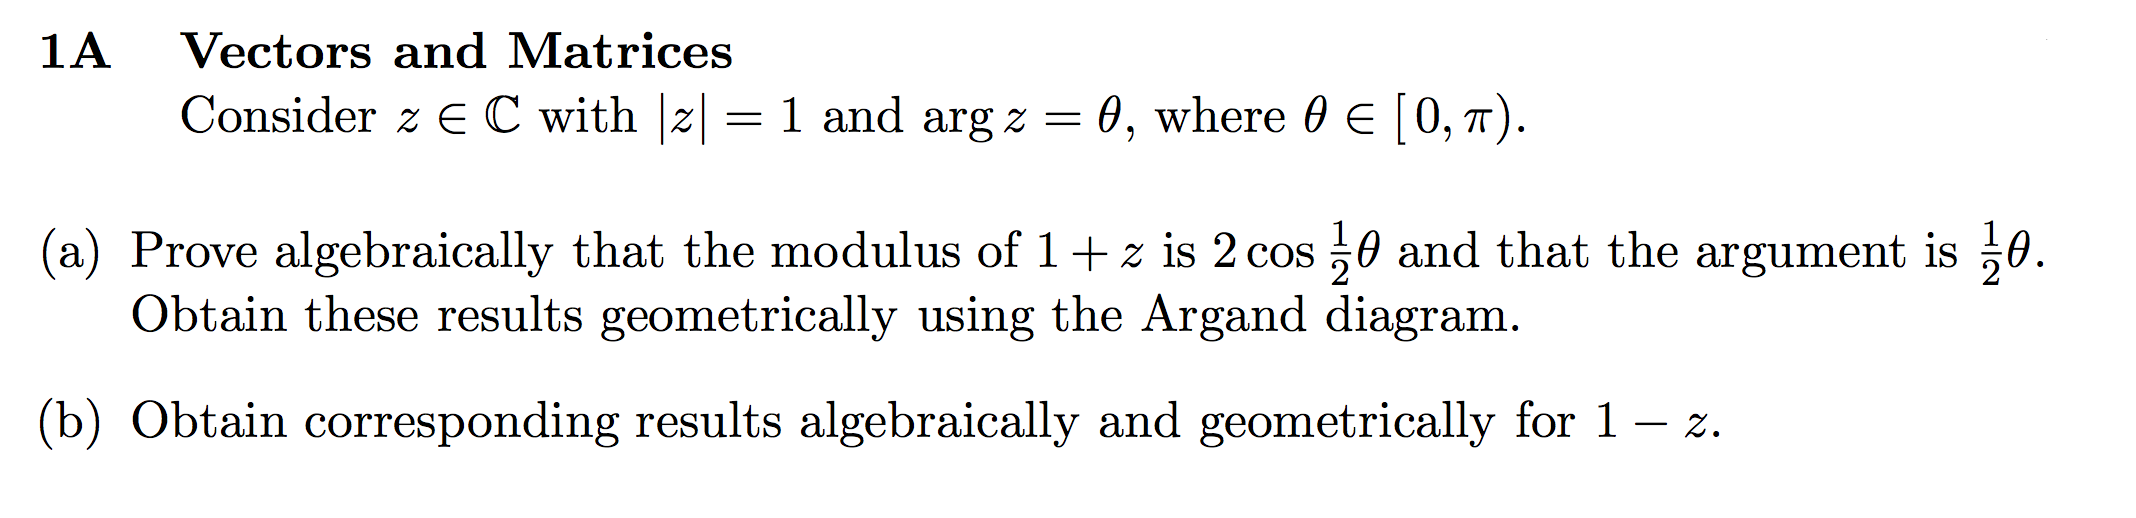
\includegraphics[width=400pt]{img/misc--cambridge-1a-2017-1-1A.png}
\end{mdframed}
\begin{proof}(Algebraic)\\
Note that
$\cos\theta = \cos^2\frac{1}{2}\theta - \sin^2\frac{1}{2}\theta = 2\cos^2\frac{1}{2}\theta - 1$.

We have $z = \cos\theta + i\sin\theta$ and therefore
\begin{align*}
  |1 + z|  &= \sqrt{(1 + \cos\theta)^2 + \sin^2\theta}
             = \sqrt{2(1 + \cos\theta)}
             = \sqrt{2\Big(1 + 2\cos^2\frac{1}{2}\theta - 1\Big)}
             = 2\cos\frac{1}{2}\theta\\
  |1 - z| &= \sqrt{(1 - \cos\theta)^2 + \sin^2\theta}
            = \sqrt{2(1 - \cos\theta)}
            = \sqrt{2(1 - (2\cos^2\frac{1}{2}\theta - 1))}
            = 2\sin\frac{1}{2}\theta.
\end{align*}
\end{proof}

\begin{proof}(Geometric)\\
  \begin{mdframed}
    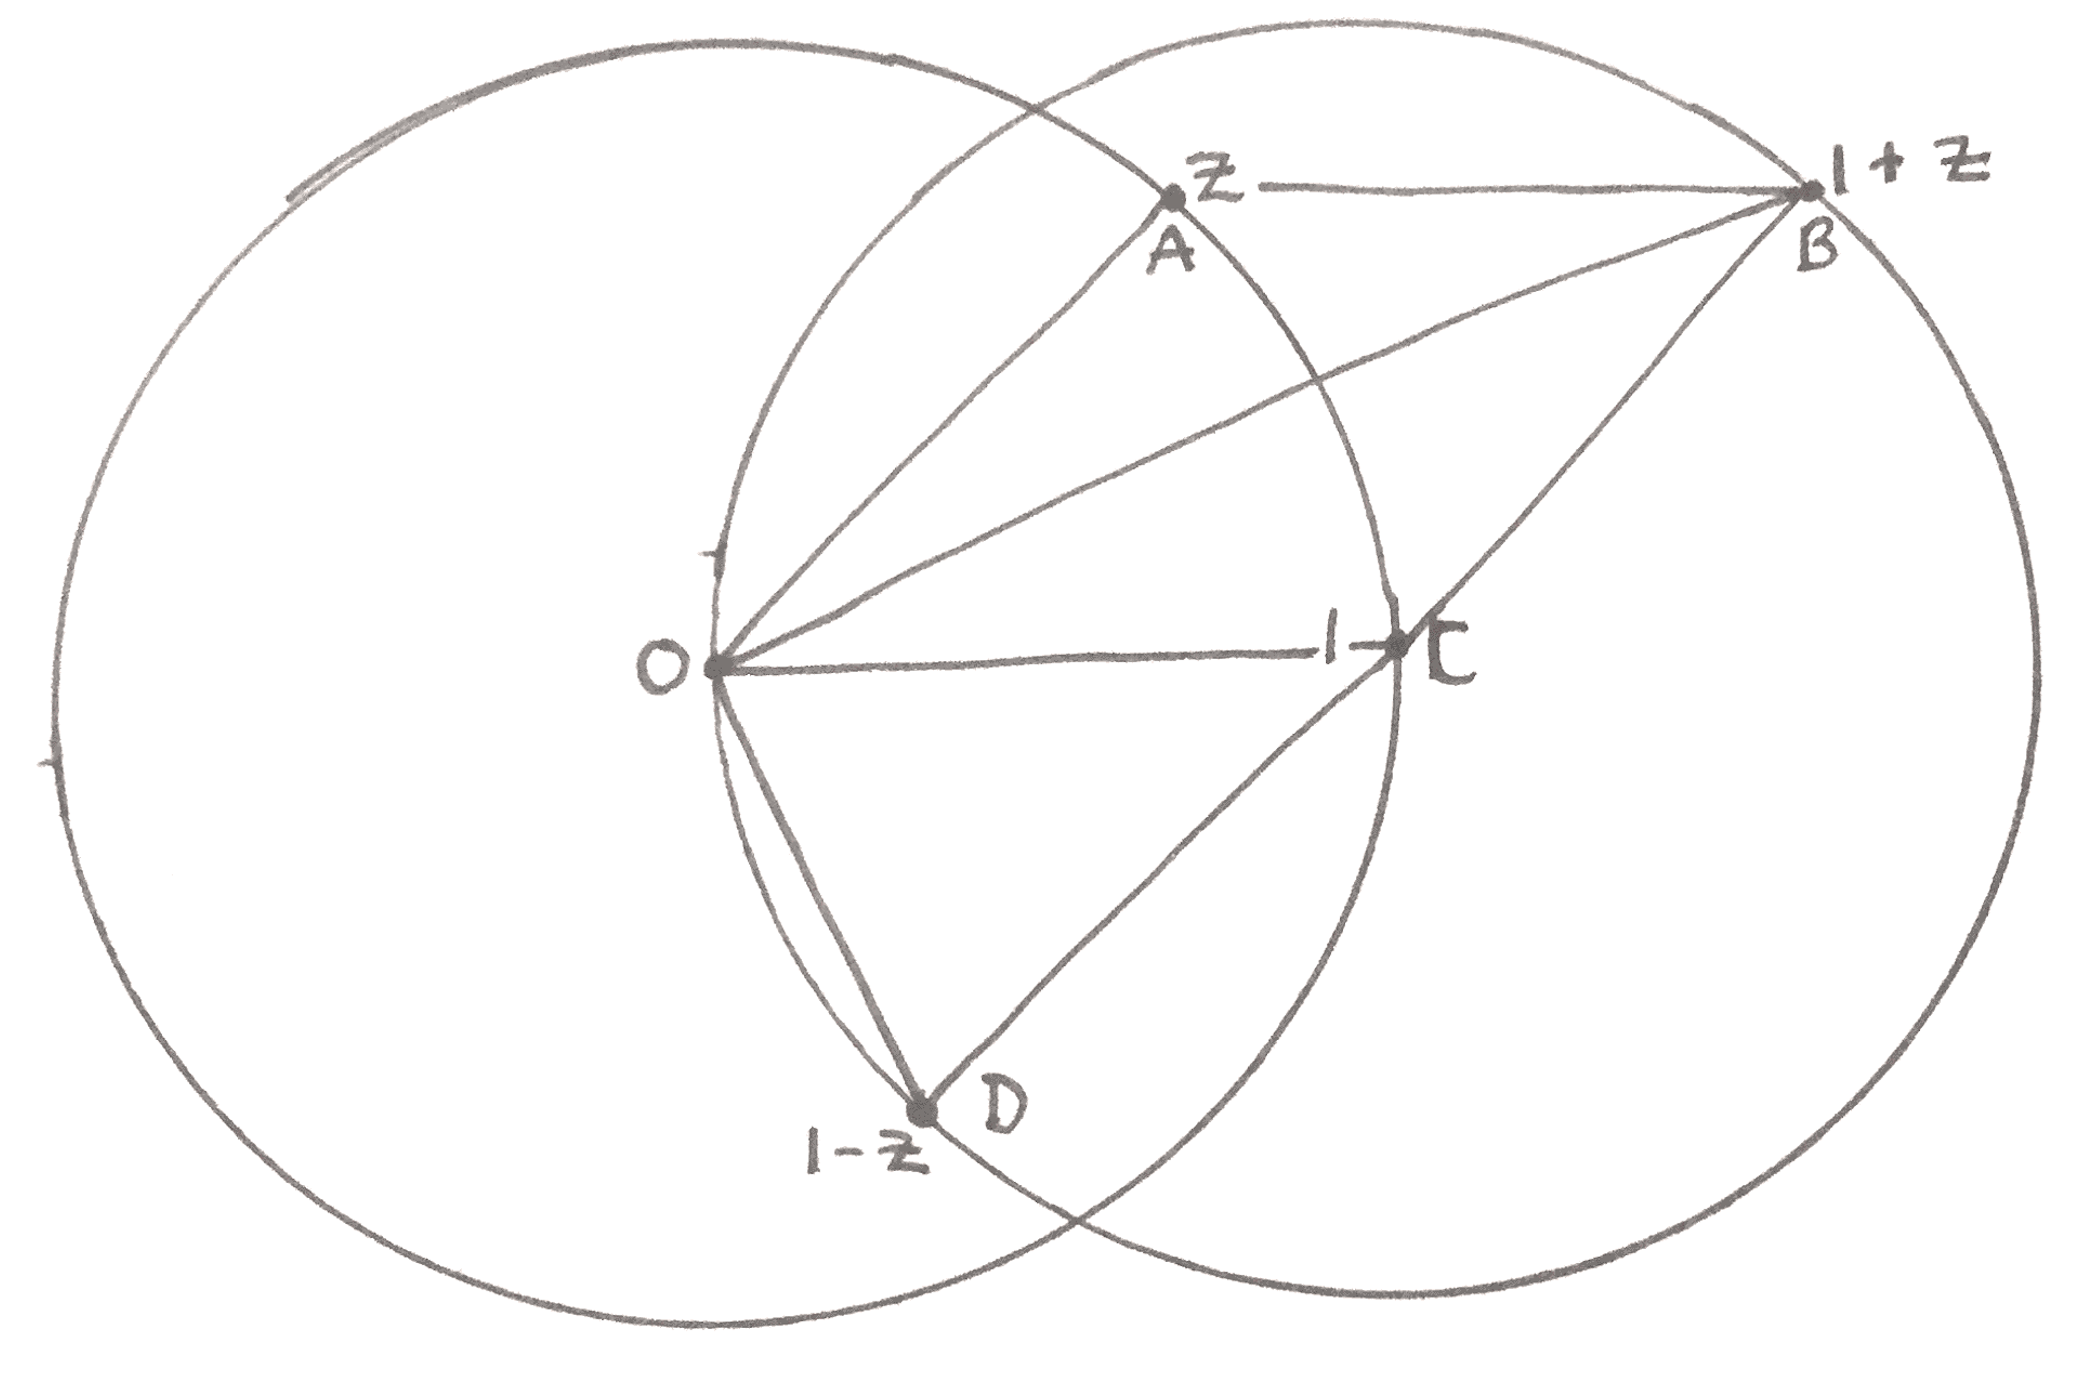
\includegraphics[width=300pt]{img/misc--cambridge-1a-2017-1-1A-diagram.png}
  \end{mdframed}
  $OABC$ is a rhombus, with sides of length 1 and $\angle AOC=\theta$. The diagonal $OB$ bisects
  $\angle AOC$, therefore $\angle OBC = \theta/2$. $\angle BOD$ is a right angle since it is formed
  from a triangle inscribed in a circle. Hypotenuse $BD$ has length 2, since $C$ is the centre of a
  second unit circle with radii $CB$ and $CD$. Therefore the length of $OB$ is
  $2\cos\frac{1}{2}\theta$ and the length of $OD$ is $2\sin\frac{1}{2}\theta$.
\end{proof}


\newpage
\subsection*{2C}
\begin{mdframed}
  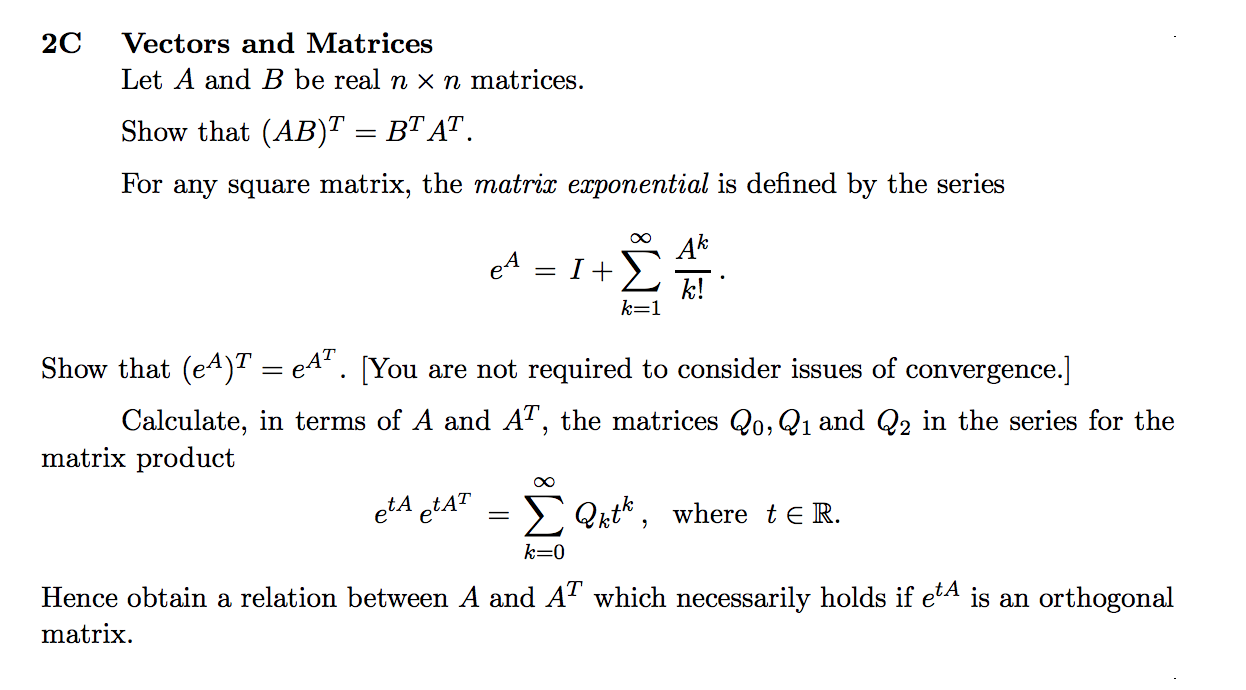
\includegraphics[width=400pt]{img/misc--cambridge-1a-2017-1-2c.png}
\end{mdframed}

\begin{claim*}
  $(AB)^T = B^TA^T$
\end{claim*}

\begin{proof}
  Let $i, j \in \{1, \ldots, n\}$. Then
  \begin{align*}
    \((AB)^T\)_{ij} = (AB)_{ji}
                   = \sum_{l=1}^n A_{jl}B_{li}
                   = \sum_{l=1}^n (A^T)_{lj}(B^T)_{il}
                   = (B^TA^T)_{ij}
  \end{align*}
\end{proof}

\begin{lemma*}
  $(A^k)^T = (A^T)^k$.
\end{lemma*}

\begin{proof}
  Note that $(A^m)^T(A^T)^n = (AA^{m-1})^T(A^T)^n = (A^{m-1})^T(A^T)^{n+1}$. By iterating this
  formal manipulation $k$ times, we have $(A^k)^T = (A^k)^T(A^T)^0 = (A^0)^T(A^T)^k = (A^T)^k$.
\end{proof}

\newpage
\begin{claim*}
  $(e^A)^T = e^{(A^T)}$
\end{claim*}

\begin{proof}
  Note that $(e^A)_{ij} := \sum_{k=0}^\infty \frac{(A^k)_{ij}}{k!}$, where $A^0 := I$ and
  $0! := 1$.  Therefore
  \begin{align*}
    \((e^A)^T\)_{ij} = \sum_{k=0}^\infty \frac{((A^k)^T)_{ij}}{k!}
                    = \sum_{k=0}^\infty \frac{((A^T)^k)_{ij}}{k!}
                    = \(e^{(A^T)}\)_{ij} .
  \end{align*}
\end{proof}

\begin{problem*}
  For $t \in \R$ we define matrices $Q_k$ such that $e^{tA}e^{tA^T} = \sum_{k=0}^\infty
  Q_kt^k$. Calculate $Q_0, Q_1, Q_2$.
\end{problem*}

\begin{proof}[Solution]~\\
  We switch notation, so that $Q_k$ becomes $Q^{(k)}$. We have
  \begin{align*}
    \(e^{tA}e^{tA^T}\)_{ij}
    &=
      \(\sum_{k=0}^\infty\frac{((tA)^k)_{ij}}{k!}\)
      \(\sum_{k=0}^\infty \frac{((tA^T)^k)_{ij}}{k!}\)\\
    &=
      \(\sum_{k=0}^\infty\frac{t^k}{k!}(A^k)_{ij}\)
      \(\sum_{k=0}^\infty \frac{t^k}{k!}(A^k)_{ji}\)\\
    &= \delta_{ij}\delta_{ji}t^0
      + (A_{ij}\delta_{ji} + \delta_{ij}A_{ji})t
      + \(A_{ij}A_{ji} + \frac{1}{2}\delta_{ij}A^2_{ji} + \frac{1}{2}A^2_{ij}\delta_{ji}\)t^2 + \ldots\\
    &= Q^{(0)}_{ij}t^0 + Q^{(1)}_{ij}t + Q^{(2)}_{ij}t^2 + \ldots.
  \end{align*}
  Therefore
  \begin{align*}
    Q_0 &= I\\
    Q_1 &= 2\diag(A)\\
    Q_2 &= AA^T + \frac{1}{2}\diag(A^2).
  \end{align*}

  If $e^{tA}$ is orthogonal, then
  $e^{tA}e^{tA^T} = e^{tA}(e^{tA})^\1 = I = \sum_{k=0}^\infty Q_kt^k$.
\end{proof}

\newpage
\subsection*{3F}
\begin{mdframed}
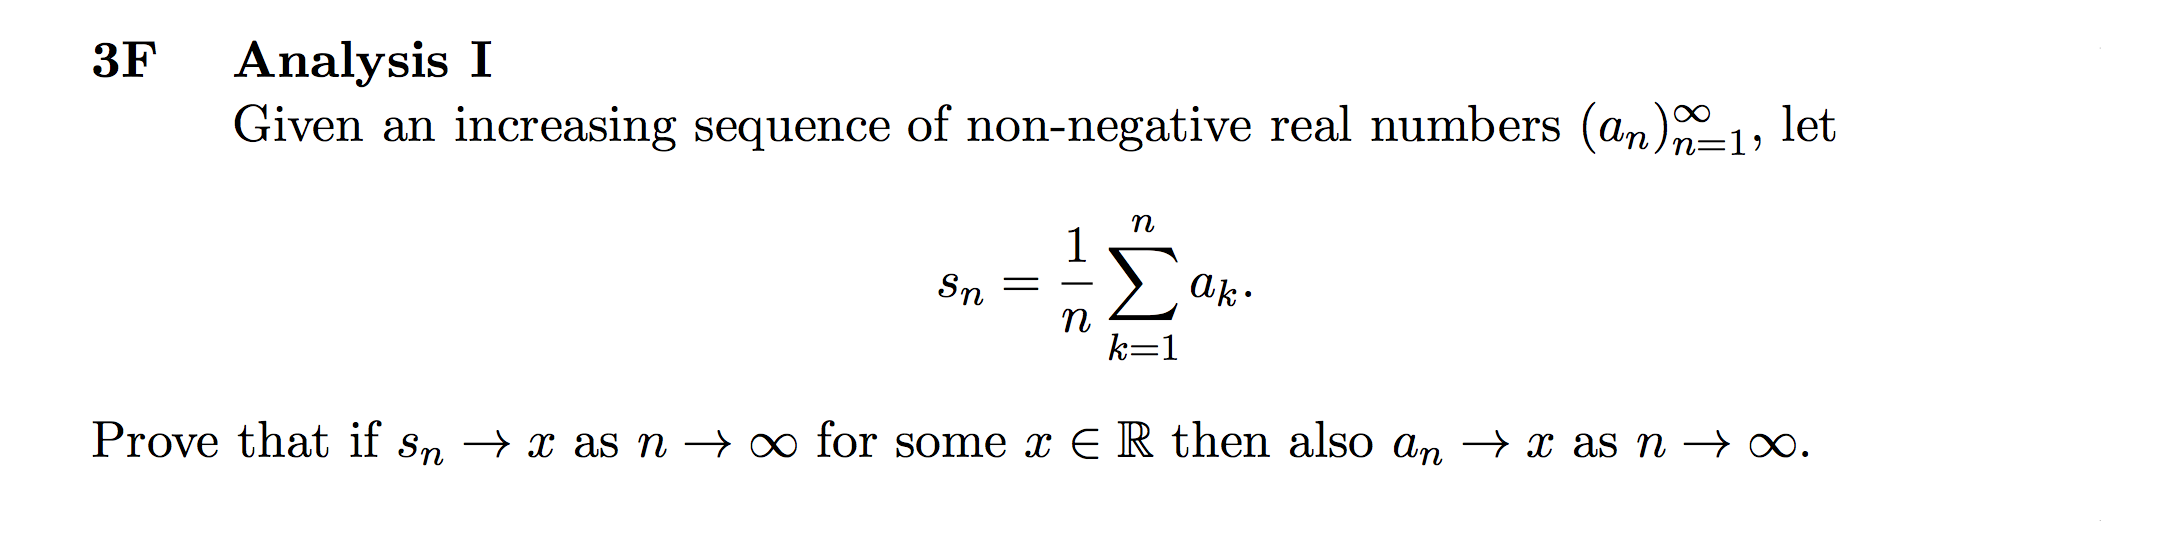
\includegraphics[width=400pt]{img/misc--cambridge-1a-2017-1-3f.png}
\end{mdframed}

\begin{proof}
  Assume that $s_n \to x$ as $n \to \infty$. We will show that $s_n \leq a_n \leq x$, for all $n$,
  therefore $a_n \to x$ as $n \to \infty$, as required.

  First note that $s_{n+1} = \frac{n}{n+1}s_n + \frac{1}{n+1}a_{n+1}$.
  % Note that $s_{n+1} = \frac{1}{n+1}\(\sum_{k=1}^na_k + a_{n+1}\) = \frac{n}{n+1}s_n + \frac{1}{n+1}a_{n+1}$.

  We now show that $s_n \leq a_n$ for all $n$. It is true for $n = 1$; assume for induction that
  it's true for $n = k$. Then we have
  $s_{k+1} = \frac{k}{k+1}s_k + \frac{1}{k+1}a_{k+1} \leq \frac{k}{k+1}a_k + \frac{1}{k+1}a_{k+1}
  \leq a_{k+1}$, as required.

  Finally we show that $a_n \leq x$ for all $n$. Seeking a contradiction, assume that there exists
  $M$ such that $a_M > x$. Let $\epsilon = a_M - x > 0$.

  % Since $(a_n)$ is increasing, we have $a_n - x \geq \epsilon$ for all $n \geq M$.

  Define
  $\Delta_n := s_{n+1} - s_n
             = \frac{n}{n+1}s_n + \frac{1}{n+1}a_{n+1} - s_n
             = \frac{1}{n+1}(a_{n+1} - s_n)
             > \frac{1}{n+1}(x + \epsilon - s_n)
             $.

  Now, we seek $N \geq M$ such that $x - s_N < \Delta_N$, since then we will have $s_{N+1} > x$, a
  contradiction. Solving for such an $N$, we have
  \begin{align*}
    x - s_N &< \frac{1}{N+1}(x + \epsilon - s_N)\\
    s_N\frac{N}{N+1} &> x\frac{N}{N+1} - \frac{\epsilon}{N+1}\\
    s_N &> x  - \epsilon/N.
  \end{align*}
  Hm, but we require an expression for $s_N$ that does not depend on $N$. Let's try $\epsilon/M$.

  Let $N$ be such that $x - s_N < \epsilon/M$. Then
  \begin{align*}
   \Delta_N &> \frac{1}{N+1}(\epsilon + \epsilon/M)\\
            &=\epsilon/M - \frac{N}{N+1}\epsilon/M + \frac{1}{N+1}\epsilon\\
            &= \epsilon/M - \epsilon\(\frac{N}{M(N+1)} - \frac{1}{N+1}\),
  \end{align*}
  which fails to prove the desired $\Delta_N > \epsilon/M$.

  % Now let $N \geq M$ be such that $x - s_N < \epsilon$

  % Now, since each $a_n$ contributes more than $x + \epsilon$ to the running average $s_n$, there
  % must exist a point at which $s_n$ is sufficiently close to $x$ that $s_{n+1}$ will exceed
  % $x$. This will be the contradiction we seek.

  % \begin{align*}
  %   S_{N+1} &> x\\
  %   \frac{N}{N+1}s_N + \frac{1}{N+1}a_{N+1} &> x\\
  %   \frac{N}{N+1}s_N + \frac{1}{N+1}(x + \epsilon) &> x\\
  %   Ns_N + \epsilon   &> Nx\\
  %   s_N + \frac{\epsilon}{N}   &> x\\
  % \end{align*}



  % Now, let $N \geq M$ be such that $x - s_N < \epsilon/M$ (such an $N$ must exist since
  % $s_n \to x$, and $s_n$ is increasing therefore it approaches this limit from below). Then we have
  % \begin{align*}
  %   s_{N+1}      &= \frac{N}{N+1}s_N + \frac{1}{N+1}a_{N+1}\\
  %                &> \frac{N}{N+1}(x - \epsilon/M) + \frac{1}{N+1}(x + \epsilon)\\
  %                &= x + \frac{\epsilon}{N+1}\(1 - \frac{N}{M}\).
  % \end{align*}



  % \begin{align*}
  %   s_{k+1} &= \frac{k}{k+1}s_k + \frac{1}{k+1}a_{k+1}\\
  %           &\leq \frac{k}{k+1}a_k + \frac{1}{k+1}a_{k+1}\\
  %           &\leq a_{k+1},
  % \end{align*}
  % as required.


  % Fix $\epsilon > 0$ and let $N$ be such that $|x - s_n| < \epsilon$ for all $n \geq N$. (Such an
  % $N$ exists by the definition of limit.) We show below that the same $N$ works for $(a_n)$. That
  % is $|x - a_n| < \epsilon$ for all $n \geq N$. Therefore $a_n \to x$ as $n \to \infty$, as
  % required.

  % Suppose that $a_n \geq x$ for some $n$.



  % \textbf{Proof that $|x - a_n| < \epsilon$ for all $n \geq N$}\\
  % Note that, since the sequence $(a_n)$ is increasing:
  % \begin{enumerate}
  % \item The sequence $(s_n)$ is also increasing (since $s_n$ is the average of $a_1, \ldots, a_n$).
  % \item $s_n < x$ for all $n$ (since $(s_n)$ approaches its limit from below).
  % \item $s_n \leq a_n$ for all $n$ (since $s_n$ is an average of numbers not greater than $a_n$).
  % \item $a_n < x$ for all $n$ (since if any $a_n \geq x$ then ...)
  % \end{enumerate}



  % Recall that we have $|x - s_n| < \epsilon$ for all $n \geq N$.

  % Therefore $x - s_n < \epsilon$ for all $n \geq N$, since $s_n < x$.

  % Therefore $x - a_n < \epsilon$ for all $n \geq N$, since $s_n \leq a_n < x$.
\end{proof}

% Since $s_n \to x$ as $n \to \infty$ we have
% \begin{enumerate}
% \item $\forall \epsilon > 0 ~ \exists N: \forall n > N: |s_n - x| < \epsilon$
% \end{enumerate}
% \begin{align*}
%   |s_n - x| < \epsilon\\
%   \Big|\frac{1}{n}\sum_{k=1}^na_k - x\Big| < \epsilon\\
% \end{align*}

\end{document}
